\chapter{Dostępne systemy monitorujące}
\label{chap:Systemy}

Na rynku dostępnych jest wiele bardzo różnych systemów
monitorujących. Narzędzia z~tej grupy możemy podzielić na dwie
kategorie:

\begin{itemize}
\item Systemy dostępnościowe,
\item Systemy analityczne.
\end{itemize}

Systemy monitorujące, w~których główny nacisk położony jest na
zapewnienie ciągłej dostępności monitorowanych usług, nazywane są
systemami dostępnościowymi. Wspierają one administratora
w~codziennych zadaniach poprzez nieustanne monitorowanie aktualnego
stanu sieci. Narzędzia te są wykorzystywane przede wszystkim do
szybkiego powiadamiania oraz lokalizacji awarii.

Systemy analityczne, w~kontekście monitorowania infrastruktury
sieciowej, to systemy, które są nastawione na zbieranie i~analizę
danych o~usługach i~parametrach urządzeń. Tego typu systemy nie są
zazwyczaj wykorzystywane do powiadamiania czy lokalizacji awarii. Ich
zadaniem jest przede wszystkim gromadzenie danych dotyczących zużycia
poszczególnych zasobów, czy też wskaźników jakości poszczególnych
usług. Systemy te posiadają zazwyczaj bardzo rozbudowane narzędzia
służące do generacji i~analizy wykresów na podstawie zebranych
wcześniej danych.

Posiadanie dwóch odrębnych systemów jest niewygodne, zwłaszcza przy
monitorowaniu rozbudowanej infrastruktury. Producenci oprogramowania
monitorującego wychodząc na przeciw użytkownikom udostępniają
dodatkowe komponenty, które zmieniają klasyczny system dostępnościowy
w~hybrydowy. Pozwalają one na kompleksowe zarządzanie infrastrukturą
sieciową. Dzięki zastosowaniu takiego systemu administrator uzyskuje
jeden uniwersalny interfejs. Możliwy jest w~nim zarówno pogląd
bieżącego stan sieci oraz diagnoza awarii, jak i~analiza danych
historycznych.

Przechowywanie danych zgromadzonych podczas monitorowania może odbywać
się na różne sposoby. Podstawową techniką przechowywania danych,
w~systemach monitorujących na początku były płaskie struktury
plików. Okazało się jednak, że rozwiązanie to jest słabo skalowalne
i~utrudnia rozmieszczanie systemu na wielu urządzeniach. Ponadto
sprawne zarządzanie zgromadzonymi danymi spoza systemu monitorującego
wymaga dużego wkładu pracy własnej administratora. Rozpowszechniły się
zatem techniki przechowywania zebranych danych w~oparciu o~bazy
danych. Wykorzystuje się tu najczęściej bazy relacyjne i
cykliczne\footnote{ Istnieje kilka implementacji np. RRD --- {\em
    Round Robin Database}\cite{www:RRDtool} oraz
  Whisper\cite{www:Whisper}. Poszczególne implementacje mogą się
  znacząco różnić w~implementacji oraz dostępnych funkcjonalnościach
  dodatkowych, jednak ogólna zasada działania jest taka sama.}.

Dane przechowywane w~relacyjnych bazach danych zorganizowane są
w~postaci tabel, a~powiązania pomiędzy danymi nazywane są
relacjami. Taka organizacja bazy danych sprawia, że wraz z~upływem
czasu jej rozmiar rośnie. Powoduje to zwiększenie zajętości
przestrzeni dyskowej, a~także wpływa na czas wykonywania
operacji. Dane są przechowywane w~bazie do czasu, gdy użytkownik
jawnie je usunie. Pozwala to na przeglądanie dowolnie długiego okresu
historii bez utraty dokładności, a~także na dynamiczne zarządzanie
czasem przechowywania danych. Ponadto możliwa jest w~każdej chwili
zmiana danych z~dowolnego okresu. Narzędzia korzystające z~tego typu
baz muszą posiadać pewną politykę zarządzania zgromadzonymi danymi aby
zapobiec nadmiernej zajętości dysku. Istotne jest jednak, że polityka
ta jest uzależniona jedynie od aplikacji, a~nie od samej bazy danych
i~może być zmieniana w~dowolnym momencie.

Cykliczne bazy danych posiadają natomiast stały, definiowany podczas
tworzenia rozmiar\footnote{Trwają obecnie prace nad nową implementacją
  cyklicznej bazy danych --- Ceres\cite{www:Ceres}, która znosi to
  ograniczenie. W~chwili pisania tej pracy projekt nie był jednak w
  fazie rozwoju pozwalającej na jego wykorzystanie.}. Rozmiar ten
określa liczbę porcji danych, jaka może być przechowywana
w~bazie. Jeśli rozmiar bazy przekroczy rozmiar zadany przy tworzeniu,
wykonywana jest konsolidacja danych. Polega ona na wyliczeniu zadanych
wartości w~odpowiednich przedziałach i~zachowaniu ich w~pojedynczych
rekordach, oraz usunięcie dokładnych danych. W bazach RRD możliwe są
trzy typy konsolidacji danych: minimum, średnia oraz maksimum. Rozmiar
bazy danych jest definiowany w~chwili jej tworzenia i~późniejsza jego
modyfikacja nie jest już możliwa. Ponadto należy zwrócić szczególną
uwagę na fakt, iż dane są usuwane z~bazy danych bez wiedzy użytkownika
czy aplikacji, przez co taka baza danych nie może zostać użyta do
dokładnej analizy danych historycznych. Istotną kwestią jest, że RDD
nie pozwala na modyfikowanie danych historycznych, lecz jedynie tych
pochodzących z~bieżącego okna czasowego. Oznacza to na przykład brak
możliwości importowania do takiej bazy danych historycznych. Istnieją
jednak implementacja jak na przykład Whisper, które nie posiadają tego
ograniczenia.

W~dalszych punktach przedstawione zostały wybrane systemy
monitorowania. Podstawowym kryterium wyboru opisywanych systemów była
ich dostępność na licencji umożliwiającej przeglądanie oraz
modyfikację w~dowolny sposób jego kodu źródłowego. Ponadto zwrócono
również uwagę na popularność systemów w~środowisku administratorów,
a~także na dostępność dokumentacji. Na tej podstawie wybrano spośród
systemów analitycznych system Cacti. Spośród systemów dostępnościowych
wybrano natomiast systemy Nagios oraz Icinga.


\section[Cacti][System monitorowania Cacti]{System monitorowania Cacti}

Cacti\cite{www:Cacti} jest systemem monitorującym, rozwijanym przez The Cacti Group
Inc. i~dystrybuowanym na licencji~GPL\footnote{ ang. {\em General
    Public License} - popularna licencja oprogramowania o~otwartych
  źródłach. Treść licencji można znaleźć w~\cite{www:GPLv2}.}. System
bazuje na oprogramowaniu RRDtool\cite{www:RRDtool}. Jest to narzędzie,
które pozwala na wykorzystanie cyklicznej bazy danych RRD do
składowania pomiarów wartości w~zadanym przedziale czasowym. Ponadto
dostarcza ono funkcji do generacji wykresów w~kilku
formatach. Dokładny opis wszystkich możliwości RRDTool można znaleźć
w~\cite{www:RRDtool}. Dzięki wykorzystaniu wspomnianego narzędzia
system ma bardzo prostą budowę i~składa się z~następujących elementów:

\begin{itemize}
\item interfejsu użytkownika,
\item dostawcy danych,
\item magazynu danych.
\end{itemize}

Magazyn danych, jest to po prostu cykliczna baza danych RRD
obsługiwana przez program przy pomocy narzędzia RRDtool.

\begin{figure}[h]
\label{fig:CactiInterface}
\caption{Interfejs użytkownika systemu Cacti.}
\begin{center}
\makebox[\textwidth]{%
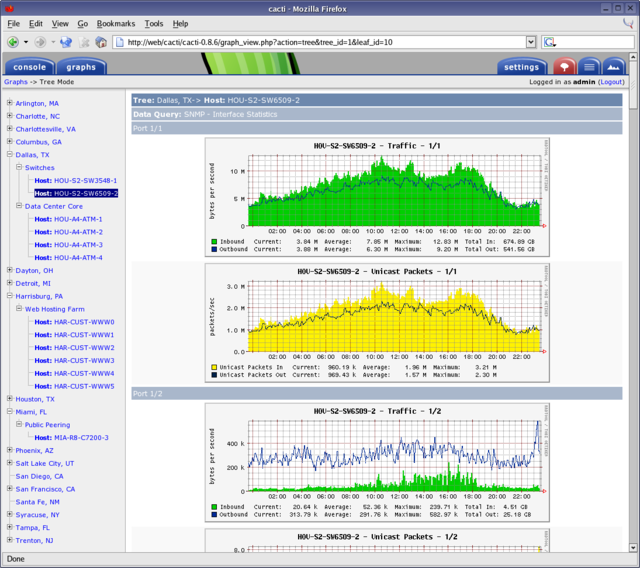
\includegraphics[width=1\textwidth]{img/cacti.png}
}\\[0.1cm]
\end{center}
\end{figure}

Interfejs użytkownika został napisany w~języku PHP. Do jego działania
niezbędny jest serwer http, np. Apache. Rysunek
\ref{fig:CactiInterface} przedstawia przykładową podstronę systemu
Cacti. Z~poziomu interfejsu użytkownika możliwa jest graficzna
konfiguracja całego systemu. Interfejs posiada klasyczną
budowę. Składa się on z~jednokolorowego paska menu, w~którym zawarte
są odnośniki do poszczególnych podstron, oraz z~pulpitu, na którym
wyświetlane są wybrane dane. Interfejs umożliwia graficzne
przedstawienie wyników w~postaci wykresów. Format wykresu może być
definiowany bezpośrednio przez użytkownika lub można skorzystać
z~bogatej biblioteki gotowych szablonów. Dostęp do interfejsu
zabezpieczony jest przez mechanizm uwierzytelnienia użytkownika
systemu monitorującego. Możliwe jest definiowanie wielu użytkowników
oraz ich uprawnienia. Każdy użytkownik ma możliwość definiowania
własnego zestawu wykresów oraz pulpitów.

Dostawca danych to element systemu, który jest odpowiedzialny za
faktyczne wykonywanie sprawdzeń (ang. {\em check}) aktualnej wielkości
danego parametru i~przekazywanie ich do narzędzia RRDTool. System
umożliwia wybór jednego z~dwóch dostawców danych. Pierwszym z~nich
jest {\em cmd.php}, który jest prostym skryptem napisanym w~języku
PHP. Umożliwia on monitorowanie aktywne urządzeń przy pomocy protokołu
SNMP.  Możliwe jest jedynie wykorzystanie prostego pobierania danych z
użyciem tego protokołu. Mechanizm pułapek nie jest obsługiwany. Skrypt
{\em cmd.php} przeznaczony jest do monitorowania jedynie niewielkich
sieci. Ze względów wydajnościowych nie jest możliwe wykorzystanie go
do monitorowania rozległej infrastruktury.

Drugim z~możliwych dostawców danych jest narzędzie {\em Spine},
nazywane również: {\em Cactid}. Jest to program napisany w~języku~C,
który uruchomiony jest jako serwis systemowy na urządzeniu
monitorującym. Umożliwia on monitorowanie urządzeń zarówno poprzez
protokół SNMP, jak i~z~wykorzystaniem innych metod. Możliwość
dostarczenia własnych metod monitorowania opiera się na dostarczeniu
skryptu lub pliku wykonywalnego, który będzie cyklicznie uruchamiany
przez {\em Cactid}, a~jego wyniki przekazywane w~taki sam sposób, jak
ze~sprawdzeń opierających się na SNMP.

Żaden z~dostawców danych nie umożliwia monitorowania danego urządzenia
lub usługi w~sposób pasywny. Cacti nie posiada również żadnego
mechanizmu, który pozwoliłby na monitorowanie sieci w~sposób
rozproszony. Oznacza to, iż administrator musi zmienić konfigurację
sieci tak, aby jeden serwer miał dostęp do każdego urządzenia, lub
konfigurować i~zarządzać osobną instancją w~każdym segmencie. Jest to
bardzo niewygodne i~wręcz uniemożliwia monitorowanie rozległych sieci
przy pomocy Cacti.

\section[Nagios][System monitorowania Nagios]{System monitorowania Nagios}

Nagios\cite{www:Nagios} został opublikowany w~1999 roku na licencji GPL. System od
niemal 15 lat jest ciągle rozwijany i~udoskonalany zarówno przez
autorów, jak i~przez szeroką społeczność. W~systemie Nagios najwyższym
priorytetem jest kontrola bieżącej dostępności wszystkich
monitorowanych usług. Organizacja systemu zakłada, iż w~sieci znajdują
się urządzenia (ang. {\em hosts}), które mogą świadczyć pewne usługi
(ang. services)\footnote{W nomenklaturze systemu Nagios usługą
  (ang. service) nazywana jest zarówno monitorowana usługa zewnętrzna
  jak np. DNS czy FTP lecz również dowolny parametr tego urządzenia
  jak zużycie procesora czy pamięci.}. Każde urządzenie i~usługa może
  znajdować się w~jednym z~trzech stanów logicznych:

\begin{description}
\item[OK] usługa działa poprawnie,
\item[WARNING] monitorowane parametry przekroczyły stan ostrzegawczy,
\item[CRITICAL] parametry usługi przekroczyły stan krytyczny, usługa
  lub urządzenie nie funkcjonuje.
\end{description}

System posiada rozbudowane algorytmy określania stanu każdego
urządzenia oraz usługi. Działanie usługi jest zawsze zależne od stanu
urządzenia, na którym dana usługa jest świadczona. Ponadto użytkownik
może definiować zależności pomiędzy urządzeniami, np. komunikacja
z~danym serwerem jest uzależniona od funkcjonowania routerów
znajdujących się na trasie pakietów.

Określanie stanu usługi odbywa się przy pomocy zewnętrznych programów
nazywanych wtyczkami (ang. {\em plugin}). W~ramach projektu {\em
  Nagions Plugins}\cite{www:NagiosPluginProject} dostępna jest bardzo
duża liczba wtyczek, dzięki czemu system Nagios może monitorować
w~sposób aktywny wszystkie podstawowe usługi. Programy znajdujące się
w~zestawie pozwalają na badanie usług takich jak HTTP, POP3, SMTP czy
FTP oraz pobierać dane o~urządzeniu przy pomocy protokołu
SNMP. Możliwe jest również napisanie własnych programów lub skryptów,
które zostaną wykorzystane jako wtyczki. Konieczne jest jednak, aby
programy te spełniały wymagania opisane
w~\cite{www:NagiosPluginsTutorial}.

Monitorowanie aktywne usług odbywa się poprzez cykliczne wykonywanie,
co zdefiniowany okres czasu wskazanej wtyczki. Wtyczka otrzymuje dla
każdego urządzenia i~usługi indywidualny zestaw parametrów wywołania,
zdefiniowany przez administratora w~plikach konfiguracyjnych
systemu. Na podstawie parametrów wywołania oraz aktualnego stanu
usługi program określa logiczny stan usługi i~przekazuje go do systemu
Nagios wraz z~dodatkowym napisem opisującym stan danej usługi. Napis
ten powinien mieć co najmniej jedną linię tekstu i~nie więcej niż
8KB. Opis formatowania tego napisu został zawarty
w~\cite{www:NagiosPluginsTutorial}. 

Możliwe jest również monitorowanie usług w~sposób pasywny. Odbywa się
ono poprzez dostarczenie przez dowolny program zewnętrzny odpowiednio
sformatowanych wyników do systemu monitorującego. Format tych danych
jest spójny z~formatem przekazywania danych z~wtyczki, jednak został
on wzbogacony o~informacje o~czasie wykonania sprawdzenia oraz dane
pozwalające na określenie, której usługi i urządzenia dotyczy dane
sprawdzenie. Dzięki udostępnieniu tej funkcjonalności system Nagios
może korzystać na przykład z~mechanizmu pułapek w~protokole SNMP.

Monitorowanie parametrów urządzeń innych niż to, na którym uruchomiony
jest system Nagios, wymaga użycia protokołu SNMP lub obecności na
danym systemie odpowiedniego agenta. Wraz z systemem Nagios dostępnych
jest wiele dodatków (ang. addon)\footnote{Należy zwrócić uwagę na
  różne znaczenie słów: "wtyczka" (ang. {\em plugin}) oraz "dodatek"
  (ang. {\em addon})}, które udostępniają takie agenty.

Monitorowanie aktywne tych parametrów może się odbyć na przykład przy
pomocy dodatku NRPE ({\em Nagios Remote Plugin Executor}). Składa się
on z dwóch części: agent oraz klient. Agent, jest to demon, który
uruchomiony jest na zdalnym (ang. {\em remote}) urządzeniu i~oczekuje
na żądania od klientów. Klient, jest to natomiast program, który
uruchamiany jest przez system Nagios jako wtyczka. W ramach swojego
wykonania program ten komunikuje się ze wskazanym demonem i~zleca mu
wykonanie danej wtyczki. Istotne jest, że wtyczka, która ma być
wykonana musi zostać wcześniej dostarczona przez administratora na
urządzenie, na którym znajduje się demon. Wynik wykonania wtyczki na
zdalnej maszynie zostanie przesłany do klienta, który przekaże dalej
ten wynik do systemu Nagios.

Monitorowanie pasywne parametrów urządzenie zdalnego może się odbywać
przy pomocy dowolnego programu uruchomionego na tym urządzeniu. Do
przekazania wyników tego monitorowania do systemu monitorującego można
natomiast użyć dodatku NSCA ({\em Nagios Service Check
  Acceptor}). Składa się on z dwóch części: serwera oraz
klienta. Serwer uruchomiony jest na tym samym systemie, co Nagios
i~oczekuje na dane. Klient natomiast, uruchamiany jest przez dodatkowy
mechanizm monitorujący na zdalnym urządzeniu w~celu przekazania
wyników pasywnego sprawdzenia do Nagiosa, kiedy jest to
potrzebne. Szerokie omówienie dodatku NSCA zostało zawarte
w~\ref{sec:NSCA}.

System Nagios posiada rozbudowany system powiadamiania administratora
o~wystąpieniu awarii oraz o~jej zakończeniu lub innych zdefiniowanych
wydarzeniach systemowych. Możliwe jest powiadamianie zarówno poprzez
email jak i~sms. Ponadto możliwe jest automatyczne wykonywanie
programów lub skryptów, jeśli wystąpiło jakieś zdarzenie. Podstawowa
wersja systemu składa się z~następujących elementów:

\begin{itemize}
\item interfejs graficzny,
\item rdzeń monitorujący,
\end{itemize}

%czy prawa autorskie?
\begin{figure}[h]
\label{fig:NagiosInterface}
\caption{Interfejs użytkownika systemu Nagios.}
\begin{center}
\makebox[\textwidth]{%
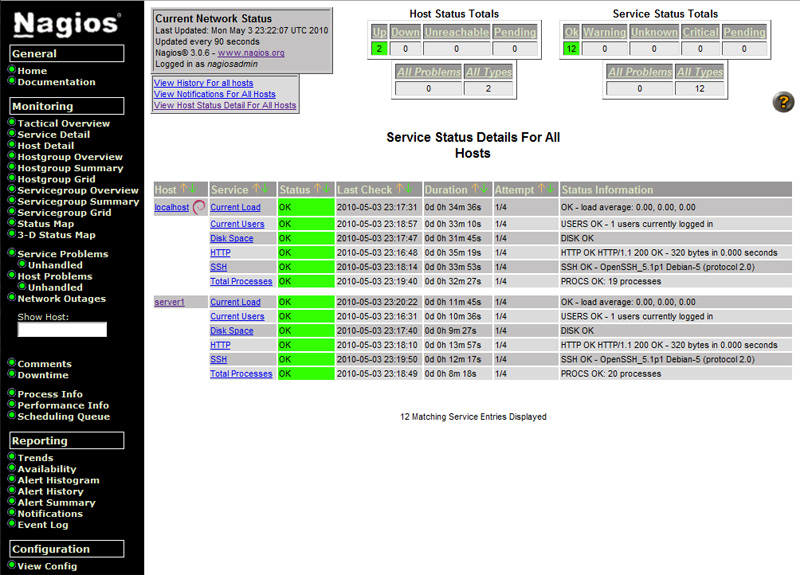
\includegraphics[width=1\textwidth]{img/nagios.jpg}
}\\[0.1cm]
\end{center}
\end{figure}

Interfejs graficzny został napisany w~języku~C z~wykorzystaniem
technologi CGI\footnote{{\em Common Gateway Interface} --
  znormalizowany interfejs służący do komunikacji pomiędzy serwerem
  www, a~zewnętrznymi programami. Interfejs ten jest wykorzystywany do
  generowania stron internetowych na żądanie klienta. Zewnętrzny
  program generuje stronę w~języku HTML, a~następnie serwer przesyła
  ją do klienta poprzez serwer http. Szczegółowy opis można znaleźć
  w~\cite{www:CGI}}. Jego wygląd jest zgodny ze~standardami z~lat 90:
klasyczna strona WWW bez dynamicznie zmieniającej się treści (patrz
rys. \ref{fig:NagiosInterface}. Dane odświeżane są na żądanie klienta
lub co określony czas. Wykorzystana technologia zakłada przesyłanie za
każdym razem całego dokumentu HTML do klienta, w~związku z~czym
generowany jest nadmierny ruch sieciowy. Widok użytkownika składa się
z~kliku części. Po lewej stronie widoczne jest klasyczne menu,
umożliwiające użytkownikowi wybór treści. Na górze strony natomiast
znajduje się podsumowanie aktualnego stanu monitorowanych urządzeń
i~usług. Centralną część okna zajmuje pulpit, który prezentuje
użytkownikowi treść wybraną wcześniej z~menu. Interfejs użytkownika
umożliwia podgląd aktualnego stanu usług oraz urządzeń. Informacja ta
może być wyświetlana w~formie listy zawierającej urządzenia i~usługi
lub w~postaci mapy sieci, która pozwala na monitorowanie stanu
urządzenia w~korelacji z~jego logicznym umieszczeniem w~strukturze
sieciowej. Możliwe jest również przeglądanie historii awarii oraz
prostych wykresów stanu urządzenia lub usługi w~zadanym przedziale
czasu. Dostęp do interfejsu chroniony jest przy pomocy autoryzacji
http. Możliwe jest definiowanie wielu użytkowników, jednak tylko
z~poziomu urządzenia, na którym uruchomiony jest system
monitorujący. Należy zauważyć również, że wszyscy użytkownicy danego
typu posiadają takie same uprawnienia. Nie ma możliwości dowolnej
edycji uprawnień danej grupy czy też użytkownika.

Rdzeń monitorujący został zaimplementowany w~języku C. Jest to centrum
całego systemu, gdyż zajmuje się on przetwarzaniem wszystkich
bieżących danych monitorowania, a~następnie składowaniem ich
w~plikach. Ta cześć systemu jest odpowiedzialna za cykliczne
uruchamianie wtyczek, a~także przetwarzaniem zarówno wyników ich
wykonania oraz wyników monitorowania pasywnego przekazanych do
systemu. Dane o~stanie sieci przechowywane są w~plikach pamięci
podręcznej systemu (ang. {\em cache}).

Sposób komunikacji pomiędzy rdzeniem monitorującym, a~interfejsem
użytkownika jest bardzo sztywny. Interfejs użytkownika uzyskuje dane
o~stanie sieci z~plików pamięci podręcznej rdzenia
monitorującego. Jeśli istnieje konieczność komunikacji w~drugą stronę,
na przykład ponieważ administrator chce zmienić jakieś parametry,
konieczne jest wykorzystanie pliku komend zewnętrznych (ang. {\em
  external commands file}). Jest to potok nazwany, z~którego dane
pobiera rdzeń monitorujący i~na ich podstawie podejmuje odpowiednie
działania. Łatwo zauważyć, że metody komunikacji wymuszają
funkcjonowanie zarówno interfejsu graficznego jak i~rdzenia
monitorującego na jednym urządzeniu. Oznacza to również, że nie jest
możliwe wykorzystanie jednego interfejsu do wyświetlania danych
z~kilku równoprawnych instancji, lecz zawsze musi istnieć jedna
instancja wyróżniona, która będzie agregowała wszystkie dane.

System posiada rozbudowane możliwości monitorowania
rozproszonego. Niestety do wykonania znacznej części z~tych
konfiguracji potrzebne są elementy systemu, które są dystrybuowane na
licencjach komercyjnych wymagających zakupu praw do korzystania z
nich. Sztandarowym przykładem jest Nagios Fusion, komercyjna
wersja interfejsu użytkownika. Zapewnia ona możliwość prezentacji
w~jednym interfejsie informacji pochodzących z~wielu instancji
systemu. Istnieją również darmowe dodatki czyli programy rozszerzające
lub zmieniające funkcjonalność systemu Nagios. Przykładem takiego
dodatku może być NDOUtils, który pozwala systemowi Nagios na
wykorzystanie bazy danych MySQL zamiast płaskich struktur plikowych
lub N2RRD, który gromadzi dane z~systemu Nagios w~bazie RRD. Możliwa
jest również częściowa integracja systemu Nagios\footnote{Szczegółowe
  informacje na temat rozszerzania funkcjonalności oraz samego systemu
  można znaleźć w~\cite{www:Nagios}.}  z~dodatkami lub systemami,
które pozwalają na wizualizacje zgromadzonych danych.

\section[Icinga][System monitorowania Icinga]{System monitorowania Icinga}
\label{subsec:Icinga}

System Icinga powstał w~2009 roku jako klon (ang. {\em fork}) systemu
Nagios. System został wzbogacony o~wiele nowych elementów, a~także
poprawiono wiele błędów obecnych w~systemie Nagios. Dzięki zachowaniu
wstecznej kompatybilności wszystkie wtyczki i~dodatki systemu Nagios
mogą być wykorzystane w~systemie Icinga. Pozyskano dzięki temu bardzo
dużą bazę wtyczek, co umożliwia monitorowanie tych samych usług
i~urządzeń co protoplasta. Podstawowe zasady funkcjonowania systemu są
identyczne, jednak wprowadzono wiele ulepszeń i~architektonicznych
poprawek.

\begin{figure}[ht]
\label{fig:IcingaInterface}
\caption{Interfejs użytkownika systemu Icinga.}
\begin{center}
\makebox[\textwidth]{%
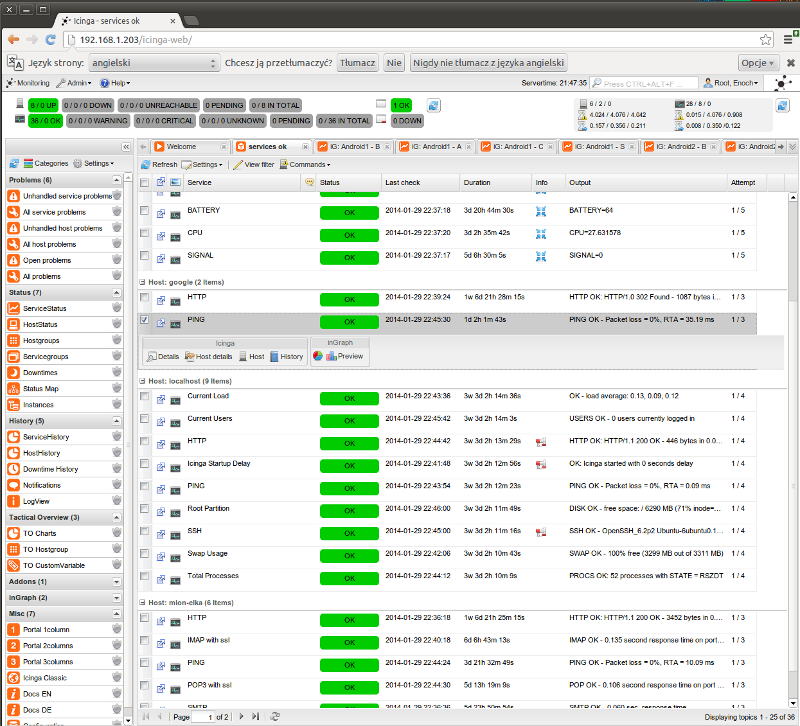
\includegraphics[width=1\textwidth]{img/icinga.png}
}\\[0.1cm]
\end{center}
\end{figure}

System Icinga został wyposażony w~zupełnie nowy interfejs
graficzny\footnote{Skorzystanie z nowego interfejsu wymaga użycia
  modułu IDOUtils oraz bazy danych. Możliwe jest wykorzystanie również
  klasycznego interfejsu, który nie posiada takich wymagań.}, który
zaimplementowano w~języku PHP przy użyciu szkieletu aplikacji
agavi\footnote{{\em Agavi } -- szkielet aplikacji języka PHP5
  pozwalający na łatwą realizację funkcjonalności zgodnej z~modelem
  programowym Model-Widok-Kontroler. Szerszy opis znajduje się na
  stronie domowej projektu: \cite{www:Agavi}}. Jest on zatem oparty na
technologii AJAX, dzięki której komunikacja z~użytkownikiem nie
opiera się na przesyłaniu całych stron w~języku HTML, lecz na
realizacji żądań generowanych poprzez język skryptowy wykonywany po
stronie użytkownika. Dzięki zastosowaniu tej technologi proces
wyświetlania strony zużywa mniejszą część pasma, a~serwer został
odciążony. Nowy interfejs użytkownika jest w~pełni dynamiczny, składa
się z~rozszerzalnego menu po lewej stronie oraz pulpitów
użytkownika w~centralnej części (patrz
rys.~\ref{fig:IcingaInterface}). Możliwe jest otwieranie wielu
pulpitów oraz wyświetlanie poszczególnych informacji w~osobnych
oknach, które można swobodnie przemieszczać w~obszarze
strony. Przykładowy pulpit dostępny dla użytkownika został
przedstawiony na rys.~\ref{fig:IcingaInterface}.

Znacznej zmianie uległ również model bezpieczeństwa. W~nowym
interfejsie graficznym każdy użytkownik posiada swój zestaw
zdefiniowanych uprawnień. Oznacza to, można ograniczyć użytkownikowi
dostęp do danych o~konkretnej usłudze lub odmówić wykonywania
niektórych czynności administracyjnych. Zarządzanie użytkownikami oraz
ich uprawnieniami możliwe jest również z~poziomu graficznego
interfejsu użytkownika, co znacząco podnosi wygodę użytkowania
systemu. Cechy te odróżniają system Icinga od systemu Nagios, w~którym
użytkownicy mogli być definiowani jedynie z~poziomu systemu
operacyjnego, na którym uruchomiony jest system monitorujący, a~ich
uprawnienia były jednakowe.

\begin{figure}[ht]
  \caption{Architektura systemu Icinga.}
  \label{fig:IcingaOverview}
  \centering
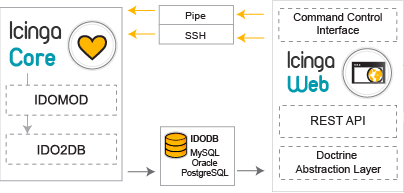
\includegraphics{img/icingaOverview.png}
\end{figure}

Kolejną istotną różnicą jest zmiana sposobu komunikacji pomiędzy
rdzeniem monitorującym a~interfejsem użytkownika. W systemie Nagios
komunikacja ta odbywała się poprzez pliki\footnote{Właściwie poprzez
  potok nazwany i~pliki.}, co uniemożliwiało wyodrębnienie interfejsu
graficznego i~umieszczenie go na oddzielnym urządzeniu. Icinga
definiuje natomiast dodatkową warstwę abstrakcji, która pozwala nowemu
interfejsowi użytkownika, na komunikację z~rdzeniem monitorującym
w~sposób niezależny od fizycznej architektury systemu. Schemat
komunikacji został przedstawiony na \ref{fig:IcingaOverview}.

Można zauważyć, że interfejs graficzny w celu pobrania danych o~stanie
bieżącym systemu, nie komunikuje się bezpośrednio z~rdzeniem lecz
poprzez REST API\footnote{ang. {\em Representational state transfer}
  -- lekka metoda przesyłania danych pomiędzy klientem
  a~serwerem.}. Na poziomie implementacji tego API poszczególne
wywołania przekładane są na abstrakcyjny język bazodanowy, a~następnie
w~zależności od typu wykorzystywanej bazy danych na właściwe pobrania
danych z~bazy. Wszystkie te operacje są dla interfejsu graficznego czy
też innego użytkownika API zupełnie przeźroczyste. Trwają obecnie
prace nad modyfikacją API, która umożliwi również przesyłanie żądań do
rdzenia monitorującego w~ten sam wygodny sposób. Obecny stan pozwala
na wysyłanie komend, które mają zostać wykonane poprzez CCI {\em
  Command Control Interface}. Implementacja tego interfejsu pozwala na
ukrycie faktycznej metody komunikacji z~rdzeniem monitorującym.

Zmiana sposobu komunikacji poszczególnych komponentów systemu, a~co za
tym idzie całej architektury pozwoliła na uzyskanie modularnej budowy
systemu. Taka architektura pozwala na wydzielenie poszczególnych
komponentów i~umieszczenie ich na odrębnych maszynach. Ponadto warstwa
abstrakcji zapewniana przez bazę danych i~API pozwala na wyświetlanie
przez jeden interfejs informacji zgromadzonych przez wiele instancji
rdzenia. Jest bardzo istotne w~przypadku rozległych sieci. Pozwala to
na rozdzielenie obciążenia wynikającego z~monitorowania na wiele
serwerów, bez konieczności istnienia instancji nadrzędnej. System
Icinga posiada również wiele innych konfiguracji rozproszonych,
a~także redundantnych. Należy również nadmienić, że wszystkie elementy
systemu potrzebne do takich konfiguracji są darmowe.

W~systemie Icinga dopracowano także możliwości współpracy
z~bazą danych. System ten pozwala na współpracę już nie tylko z~bazą
MySQL, lecz również z~bazami PostgreSQL czy bazą danych firmy
Oracle. Możliwość wykorzystania bazy danych Oracle jest bardzo
istotna, jeśli dane dotyczące konfiguracji muszą być przechowywane
przez bardzo długi czas, lub jeśli monitorowana infrastruktura jest
bardzo rozbudowana.

Warto również wspomnieć o~dostępnym dla systemu Icinga module
raportowym opartym na serwerze
JasperReports\cite{www:JasperReports}. Pozwala to w~bardzo łatwy
sposób tworzyć wzory raportów, które następnie będą automatycznie
generowane. Umożliwia to regularne i~proste tworzenie dokumentacji
niezbędnej dla zarządu przedsiębiorstwa.

\section[Podsumowanie][Podsumowanie]{Podsumowanie}

Współczesne systemy monitoringu są bardzo bogato wyposażone
i~posiadają szereg zaawansowanych możliwości. Każdy z~systemów oferuje
unikalny zestaw rozwiązań, które z~pewnością mogą zostać wykorzystane
w~wielu instytucjach. Porównując wszystkie omówione systemy, należy
zwrócić szczególną uwagę na różnice w~ich możliwych zastosowaniach
docelowych.

Systemy takie jak Cacti zaliczane są do grupy systemów
analitycznych. Ich celem jest zatem umożliwienia gromadzenia oraz
analizy danych. Zbierane dane mają charakter zagregowany w~zadanych
przedziałach, na podstawie których prezentowane są użytkownikowi
odpowiednie wykresy. Niestety ze względu na główny sposób gromadzenia
danych - protokół SNMP, oraz ubogość innych metod, systemy te nie mogą
być wzbogacone o~funkcjonalność charakterystyczną dla systemów
dostępnościowych.

Drugą grupę systemów stanowią natomiast systemy dostępnościowe, takie
jak Nagios czy Icinga. Ich głównym celem jest monitorowanie bieżącego
stanu infrastruktury i~raportowanie użytkownikowi najświeższych
informacji. Systemy te zostały również zaprojektowane w~taki sposób,
aby wspomagać administratora w~lokalizacji awarii. Głównym typem
danych, na których operują te systemy, jest stan urządzenia lub
usługi. Zdefiniowanie odpowiednich poziomów kwantyzacji dla stanów
pozwala na szybkie uzyskiwanie poglądowych informacji o~stanie
sieci. Podczas monitorowania gromadzone są również dane
szczegółowe. Ich przetwarzaniem nie zajmują się już jednak same
systemy monitorowania, lecz liczne dodatki do nich. Możliwe jest zatem
rozbudowanie systemu tego typu o~dodatkowe elementy, które pozwolą
uzyskać system hybrydowy. System taki będzie mógł pełnić rolę zarówno
systemu dostepnościowego, jak i analitycznego.

Wybierając system monitorujący należy zatem dokonać szczegółowej
analizy wymagań stawianych systemowi. Szczegółowe porównanie
wszystkich przedstawionych systemów monitorowania zawarto
w~tabeli~\ref{tab:PorownanieSys}.

\begin{longtable}[c]{|p{4.5cm}||p{3cm}|p{3cm}|p{3cm}|}
  \caption{Porównanie systemów monitorowania.} \label{tab:PorownanieSys} \\
  \hline \multicolumn{1}{|c||}{Nazwa systemu} &
  \multicolumn{1}{c|}{Cacti} & \multicolumn{1}{c|}{Nagios} &
  \multicolumn{1}{c|}{Icinga} \tabularnewline \hline \hline
  \endfirsthead

  \multicolumn{4}{c}%
  {{\tablename\ \thetable{} -- Kontynuacja z~poprzedniej strony.}} \\
  \hline
  \multicolumn{1}{|c||}{Nazwa systemu} &
  \multicolumn{1}{c|}{Cacti} & \multicolumn{1}{c|}{Nagios} &
  \multicolumn{1}{c|}{Icinga} \tabularnewline 
  \hline \hline
  \endhead

  \hline \multicolumn{4}{|r|}{{Kontynuacja na następnej stronie.}} \\ \hline
  \endfoot

  \hline\hline
  \endlastfoot

  \raggedright{Podgląd stanu bieżącego} & \raggedright{Nie} &
  \raggedright{Ta}k & \raggedright{Ta}k \tabularnewline 
  \hline

  \raggedright{Podgląd danych historycznych} &\raggedright{Tak} &
  \raggedright{Tak, przez dodatek} & \raggedright{Tak, przez dodatek}
  \tabularnewline
  \hline

  \raggedright{Dane w~formie wykresu} & \raggedright{Tak} &
  \raggedright{Tak, przez dodatek} & \raggedright{Tak, przez dodatek}
  \tabularnewline 
  \hline

  \raggedright{Przechowywanie danych w~bazie cyklicznej} & \raggedright{Tak} &
  \raggedright{Tak, przez dodatek} & \raggedright{Tak, przez dodatek}
  \tabularnewline
  \hline

  \raggedright{Przechowywanie danych w~bazie relacyjnej} & \raggedright{Nie} &
  \raggedright{Tak, przez dodatek} & \raggedright{Tak, przez dodatek}
  \tabularnewline
  \hline

  \raggedright{Powiadomienia o~awarii} & \raggedright{Nie} &
  \raggedright{Tak, email lub telefon} & \raggedright{Tak, email lub telefon}
  \tabularnewline
  \hline

  \raggedright{Wsparcie w~lokalizacji awarii} & \raggedright{Nie} &
  \raggedright{Tak, poprzez mapę logiczną sieci} & \raggedright{Tak, poprzez mapę logiczną sieci}
  \tabularnewline
  \hline

  \raggedright{Obsługa SNMP} & \raggedright{Tak} &
  \raggedright{Tak, przez wtyczkę} & \raggedright{Tak, przez wtyczkę}
  \tabularnewline
  \hline

  \raggedright{Zbieranie danych spoza SNMP} & \raggedright{Tak, niewielka liczba dostępnych metod} &
  \raggedright{Tak, bogaty zestaw wtyczek} & \raggedright{Tak, bogaty zestaw wtyczek}
  \tabularnewline
  \hline

  \raggedright{Monitorowanie pasywne} & \raggedright{Nie} &
  \raggedright{Tak} & \raggedright{Tak}
  \tabularnewline
  \hline

  \raggedright{Nowoczesny interfejs użytkownika} & \raggedright{Nie} &
  \raggedright{Nie} & \raggedright{Tak, z wykorzystaniem technologi AJAX}
  \tabularnewline
  \hline

  \raggedright{Wielu użytkowników} & \raggedright{Tak} &
  \raggedright{Tak} & \raggedright{Tak}
  \tabularnewline
  \hline

  \raggedright{Metoda uwierzytelnienia} & \raggedright{Uwierzytelnienie wewnętrzne} &
  \raggedright{Uwierzytelnienie http} & \raggedright{Uwierzytelnienie wewnętrzne}
  \tabularnewline
  \hline

  \raggedright{Zarządzanie kontami użytkowników z~interfejsu} & \raggedright{Tak} &
  \raggedright{Nie} & \raggedright{Tak}
  \tabularnewline
  \hline

  \raggedright{Definiowanie uprawnień dla użytkowników} & \raggedright{Tak, przez interfejs graficzny} &
  \raggedright{Nie} & \raggedright{Tak, przez interfejs graficzny}
  \tabularnewline
  \hline

  \raggedright{Modularność} & \raggedright{Nie} &
  \raggedright{Nie} & \raggedright{Tak}
  \tabularnewline
  \hline

  \raggedright{Rozmieszczenie modułów na różnych urządzeniach fizycznych} & \raggedright{Nie dotyczy} &
  \raggedright{Nie dotyczy} & \raggedright{Tak}
  \tabularnewline
  \hline

  \raggedright{Możliwość monitorowania rozproszonego z~instancją
    nadrzędną} & \raggedright{Nie} & \raggedright{Tak} &
  \raggedright{Tak}
  \tabularnewline
  \hline

  \raggedright{Możliwość monitorowania rozproszonego bez instancji nadrzędnej} & \raggedright{Nie} &
  \raggedright{Tak, konieczny płatny dodatek} & \raggedright{Tak}
  \tabularnewline
  \hline

  \raggedright{Generacja raportów} & \raggedright{Nie} &
  \raggedright{Nie} & \raggedright{Tak, z~wykorzystaniem JasperReports}
  \tabularnewline
  \hline

  \raggedright{Możliwość monitorowania urządzenia mobilnego} & \raggedright{Nie} &
  \raggedright{Nie} & \raggedright{Nie}
  \tabularnewline
  \hline

  \raggedright{Dostępność} & \raggedright{Darmowy} &
  \raggedright{Częściowo darmowy, wiele płatnych elementów i~funkcjonalności} & \raggedright{Darmowy}
  \tabularnewline
  \hline

  \raggedright{Licencja} & \raggedright{GPL v2} &
  \raggedright{GPL v3 (tylko darmowe elementy)} & \raggedright{GPL v2}
  \tabularnewline
  \hline

\end{longtable}

Przedstawione systemy monitorujące w~znacznym stopniu zaspokajają
zapotrzebowanie rynku na systemy monitorowania. Pojawia się jednak
pewna nisza związana z~monitorowaniem urządzeń mobilnych. Zadanie to
nie jest trywialne i~wymaga obecności dodatkowych mechanizmów zarówno
na urządzeniu mobilnym, jak i~w~innych elementach systemu. Żaden
z~analizowanych systemów nie posiadał w~swej implementacji ani
w~oficjalnych repozytoriach z~dodatkami oprogramowania, które
pozwalałoby na monitorowanie parametrów urządzenia mobilnego.

